\begin{figure}[H]
    \centering
    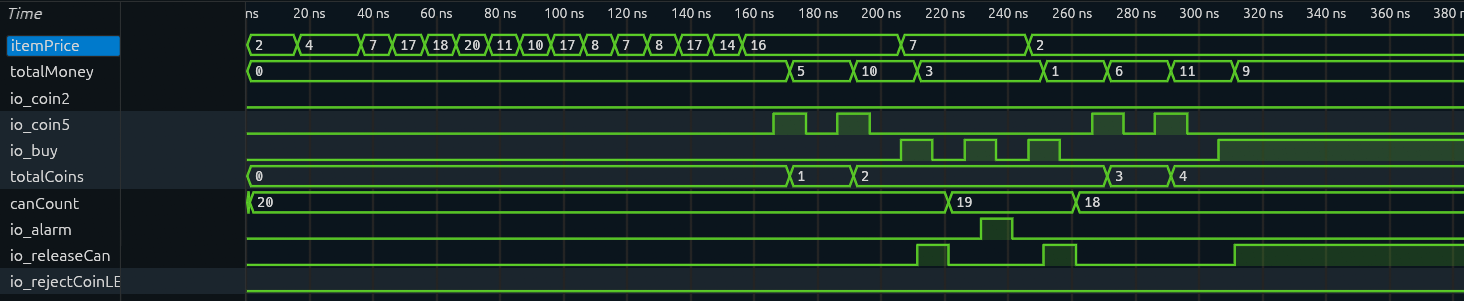
\includegraphics[width=1\linewidth]{root/Waveform_1.png}
    \caption{Waveform during Test 1(0ns -> 100ns) the different prices can be seen in \texttt{itemPrice}, Test2(100ns ->300ns) inserting coins, buying item and trying again where it is rejected.  Test3(300ns -> 500ns) Holding buy doesn't trigger multiple purchases.}
    \label{fig:placeholder}
\end{figure}
\begin{figure}[H]
    \centering
    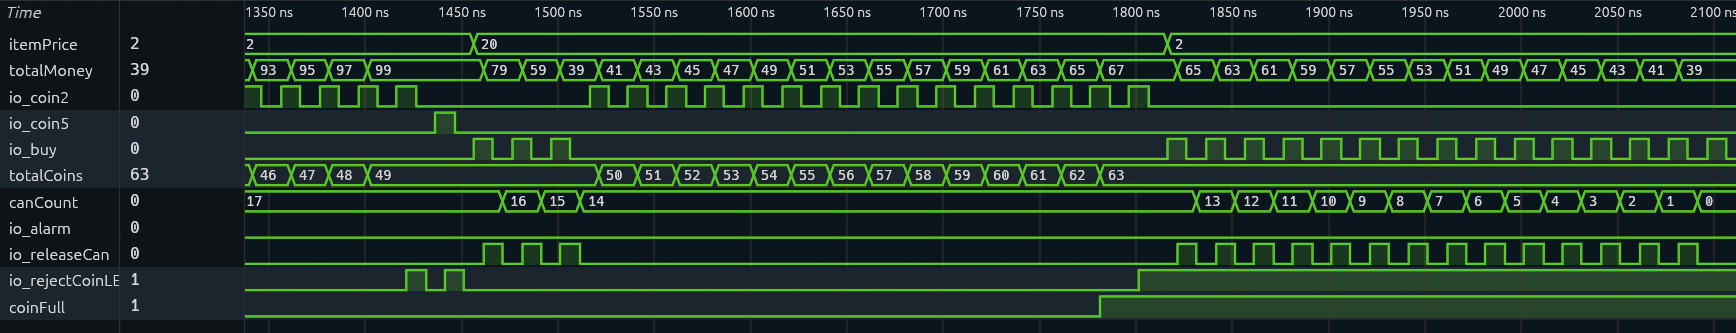
\includegraphics[width=1\linewidth]{root/Waveform_2.png}
    \caption{Test4: $\sim$1400ns checking the limit of 99kroners, not possible to insert more money, it is rejected. Test5: (1450ns-> 1800ns) inserting coins until the coin limit of 63}
    \label{fig:placeholder}
\end{figure}
\begin{figure}[H]
    \centering
    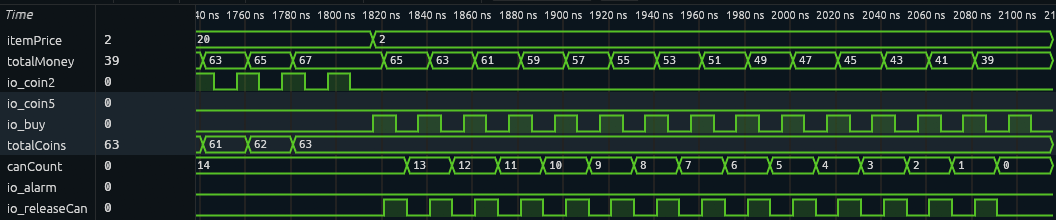
\includegraphics[width=1\linewidth]{root/Waveform_3.png}
    \caption{Test 6: (1820ns -> 2120ns) Testing if vending will release can when \texttt{canCount == 0}. releaseCan should be 0, even when trying to buy with sufficient funds.}
    \label{fig:placeholder}
\end{figure}

